\documentclass[10pt, aspectratio=169]{beamer}
\usetheme{metropolis}
\usepackage{appendixnumberbeamer}
\usepackage{booktabs}
\usepackage{graphicx}
\usepackage{amsmath}

\metroset{block=fill, progressbar=frametitle, sectionpage=none}

\definecolor{sebi}{RGB}{0, 84, 166}
\definecolor{accent2}{RGB}{220, 50, 47}
\setbeamercolor{frametitle}{bg=sebi}
\setbeamercolor{progress bar}{fg=accent2}
\setbeamercolor{alerted text}{fg=accent2}

% Caption styling
\setbeamerfont{caption}{size=\scriptsize}
\setbeamerfont{caption name}{size=\scriptsize}
\usepackage{caption}
\captionsetup{labelformat=empty} % Remove "Figure:" prefix globally for a cleaner look

\title{Determinants of Household Participation\\in Securities Markets}
\subtitle{An Empirical Analysis of the 2025 SEBI Household Survey}
\author{Shivansh Verma \and Sashwat Dhanuka}
\institute{Dept.\ of Computer Science, Ashoka University}
\date{April 2026}

\begin{document}

\maketitle

% ── SLIDE 2: Problem ──────────────────────────────────────────────────────────
\begin{frame}{The Problem}
  \begin{columns}[T]
    \begin{column}{0.52\textwidth}
      \textbf{Only 25.5\% of Indian households invest in securities.}\\[0.6em]
      Despite the post-2020 retail boom and zero-commission platforms,
      participation remains sharply stratified by socioeconomic position,
      geography, and information access.\\[0.8em]
      \textbf{Four research questions:}
      \begin{enumerate}
        \item Who is likely to participate?
        \item What keeps the 74.5\% out?
        \item Which securities do investors prefer, and for how long?
        \item Can we predict these outcomes from basic profiles?
      \end{enumerate}
    \end{column}
    \begin{column}{0.44\textwidth}
      \metroset{block=fill}
      \begin{block}{Sample}
        \begin{tabular}{lr}
          Total respondents    & 109,430 \\
          Active investors     & 27,882 (25.5\%) \\
          Non-investors        & 81,548 (74.5\%) \\
          Geographic zones     & 4 \\
          States / UTs covered & 35 \\
        \end{tabular}
      \end{block}
      \vspace{0.4em}
      \begin{block}{Methods}
        Logistic regression (HC3 robust SE, survey-weighted),
        K-means clustering, Histogram-based Gradient Boosting
      \end{block}
    \end{column}
  \end{columns}
\end{frame}

% ── SLIDE 3: Dataset ──────────────────────────────────────────────────────────
\begin{frame}{Dataset and Schema: Details}
  \textbf{Source:} 2025 SEBI Household Survey, nationally representative,
  pre-computed survey weights.\\[0.6em]
  \textbf{ETL pipeline:} 449 raw columns transformed into boolean,
  integer, and ordinal types; loaded into a normalized PostgreSQL schema
  (17 domain-specific tables anchored by \texttt{respondent\_id}).\\[0.6em]
  \textbf{Conditional routing:}
  \begin{itemize}
    \item Investors: sub-module SS\_B3 (info sources, motivations), $n = 9{,}797$
    \item Non-investors: sub-module SS\_BB2 (barriers), $n = 14{,}794$
  \end{itemize}
  All group percentages computed against the routing-eligible population.
\end{frame}

\begin{frame}{Dataset and Schema: Architecture}
  \begin{figure}
    \centering
    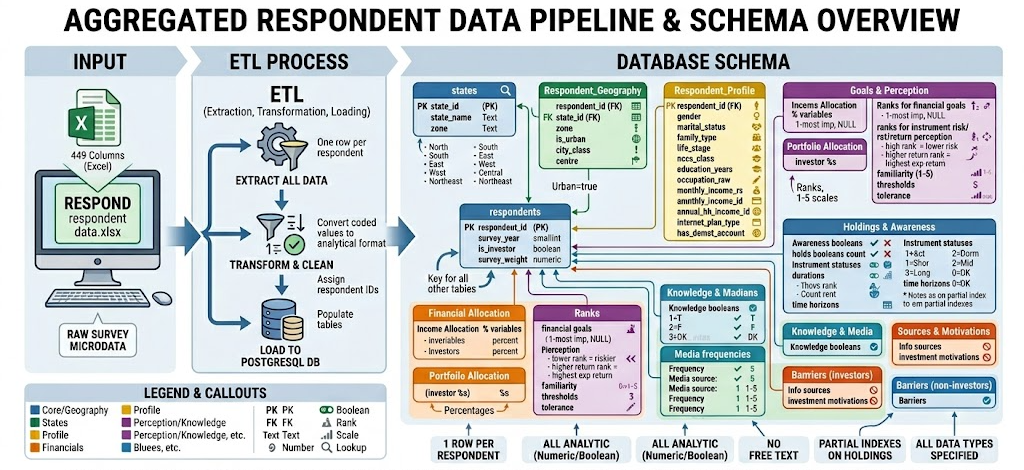
\includegraphics[height=0.8\textheight,keepaspectratio]{../figures/data_layer.png}
  \end{figure}
\end{frame}

% ── SLIDE 5: Methodology (I) ──────────────────────────────────────────────────
\begin{frame}{Methodology (I): Econometric Model}
  \textbf{Multivariate Participation Logic}
  \begin{equation*}
    \begin{aligned}
      \text{logit}(p_i) = \beta_0 &+ \beta_1 \text{Awareness}_i + \beta_2 \ln(\text{Income}_i) + \beta_3 \text{Education}_i \\
      &+ \beta_4 \text{Male}_i + \beta_5 \text{Urban}_i + \beta_6 \text{Risk}_i \\
      &+ \sum_{j} \delta_j \text{Cohort}_{ij} + \sum_{l} \lambda_l \text{Zone}_{il} + \epsilon_i
    \end{aligned}
  \end{equation*}
  \begin{itemize}
    \item \textbf{Dependent Variable:} $p_i$ is the probability of market participation ($Y=1$).
    \item \textbf{Survey Weighting:} All coefficients estimated using inverse probability weighting to match national demographics.
    \item \textbf{Robustness:} HC3 Huber-White robust standard errors to account for complex survey design and non-normality.
  \end{itemize}
\end{frame}

% ── SLIDE 6: Methodology (II) ─────────────────────────────────────────────────
\begin{frame}{Methodology (II): Unsupervised \& Predictive Layer}
  \begin{columns}[T]
    \begin{column}{0.48\textwidth}
      \textbf{Barrier Archetypes (Finding 2)}
      \begin{itemize}
        \item \textbf{Algorithm:} K-Means clustering.
        \item \textbf{Feature Space:} 18-dimensional binary vector of self-reported barriers.
        \item \textbf{Optimization:} Elbow method and Silhouette scores for cluster validation ($n=3$ archetypes).
      \end{itemize}
    \end{column}
    \begin{column}{0.48\textwidth}
      \textbf{Predictive Modeling (Layer)}
      \begin{itemize}
        \item \textbf{Model:} Histogram-based Gradient Boosting.
        \item \textbf{Capability:} Handles categorical features natively; captures complex non-linear interactions.
        \item \textbf{Validation:} 5-fold cross-validation; AUC-ROC as primary metric.
      \end{itemize}
    \end{column}
  \end{columns}
\end{frame}

% ── SLIDE 7: EDA — Participation landscape ────────────────────────────────────
\begin{frame}{EDA: Who Participates?}
  \textbf{Steepest univariate signals:}
  \begin{itemize}
    \item \alert{Income gradient:} 10.7\% (Q1, $<$Rs.\,12,500/mo)
          to 47.6\% (Q5, $>$Rs.\,35,000/mo): a \textbf{4.5$\times$} spread
    \item \alert{Gender gap:} 30.8\% (male) vs 15.8\% (female),
          persists across all income levels
    \item \alert{Urban premium:} 28.8\% vs 17.6\% (rural)
    \item Millennials (28--43) lead cohorts at 28.1\%,
          exceeding both Gen Z (24.3\%) and Gen X (22.9\%)
  \end{itemize}
  \vspace{0.8em}
  These univariate signals motivate the multivariate regression:
  which factors survive joint controls?
\end{frame}

\begin{frame}{EDA: Participation Demographics}
  \begin{figure}
    \centering
    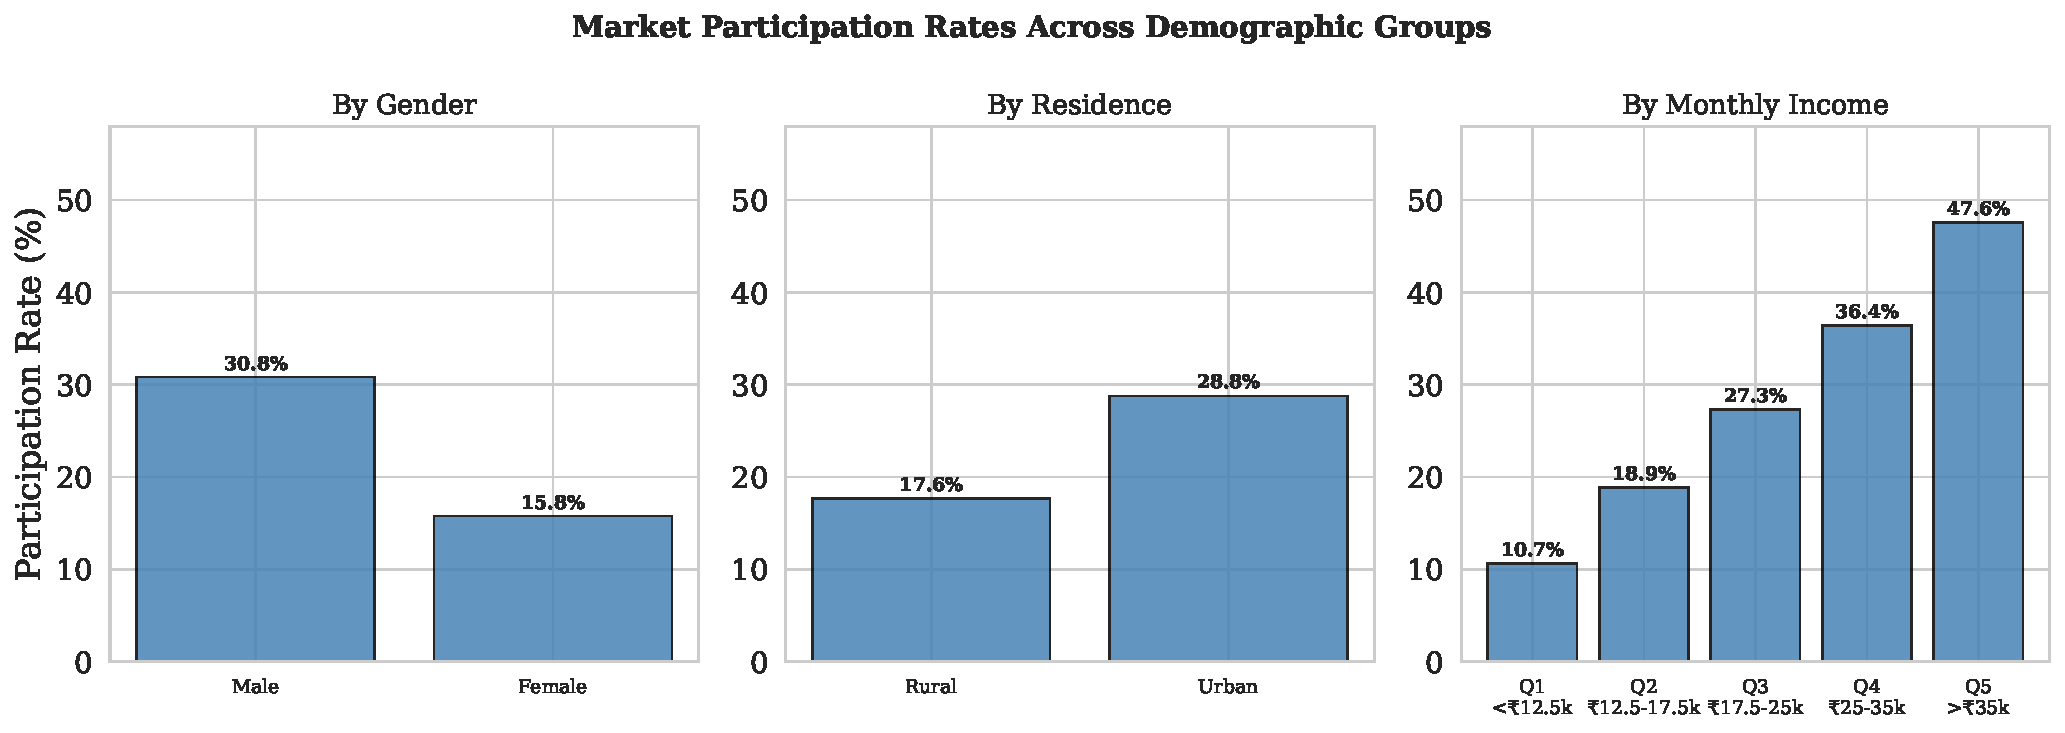
\includegraphics[height=0.65\textheight,keepaspectratio]{../figures/fig_eda1_participation_demo.pdf}
  \end{figure}
\end{frame}

% ── SLIDE 9: EDA — Awareness and holdings ─────────────────────────────────────
\begin{frame}{EDA: Awareness Gap and Holdings}
  \textbf{Awareness gradient (all 109,430 respondents):}
  \begin{itemize}
    \item Fixed Deposits: \textbf{99.1\%}
    \item Mutual Funds / ETFs: 67.0\%
    \item Direct Equity: 62.0\%
    \item Derivatives: \textbf{17.9\%}
  \end{itemize}
  \vspace{0.8em}
  \textbf{Holdings among investors:}
  \begin{itemize}
    \item MF/ETF: 66.5\% \quad FD/RD: 57.2\%
    \item Direct equity: 49.3\%
  \end{itemize}
  \vspace{0.8em}
  MFs and FDs \emph{co-dominate}: Indian retail investors layer
  market-linked products on top of traditional savings rather than
  replacing them.
\end{frame}

\begin{frame}{EDA: Instrument Awareness and Holdings}
  \begin{figure}
    \centering
    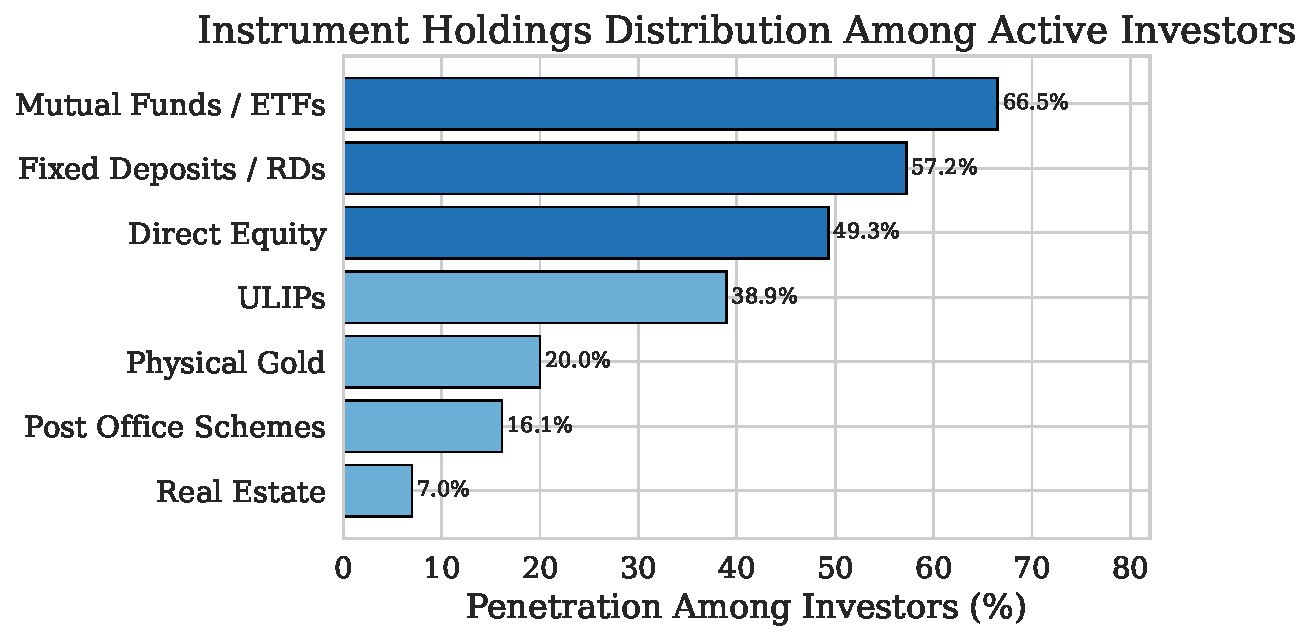
\includegraphics[height=0.8\textheight,keepaspectratio]{../figures/fig_eda2_holdings.pdf}
  \end{figure}
\end{frame}

% ── SLIDE 9: Finding 1 — Determinants of entry ───────────────────────────────
\begin{frame}{Finding 1: What Drives Market Entry?}
  \alert{\textbf{Product awareness}} is the single strongest predictor
  (OR = 2.22), exceeding:\\[0.6em]
  \begin{tabular}{ll}
    Income (log)  & OR = 1.60 \\
    Education     & OR = 1.56 \\
    Male gender   & OR = 1.53 \\
    Urban         & OR = 1.45 \\
  \end{tabular}\\[0.8em]
  Partial mediation: income and education partly work \emph{through}
  awareness, but awareness retains a large independent effect after
  SES controls.\\[0.6em]
  Two predictors return null results (Gen X, West zone):
  the model does not produce spurious significance at $N \approx 100{,}000$.
  \vspace{0.4em}
  \begin{block}{Policy implication}
    Awareness is a \textbf{distinct, actionable lever}, not merely
    an SES proxy.
  \end{block}
\end{frame}

\begin{frame}{Finding 1: Odds Ratios for Participation}
  \begin{figure}
    \centering
    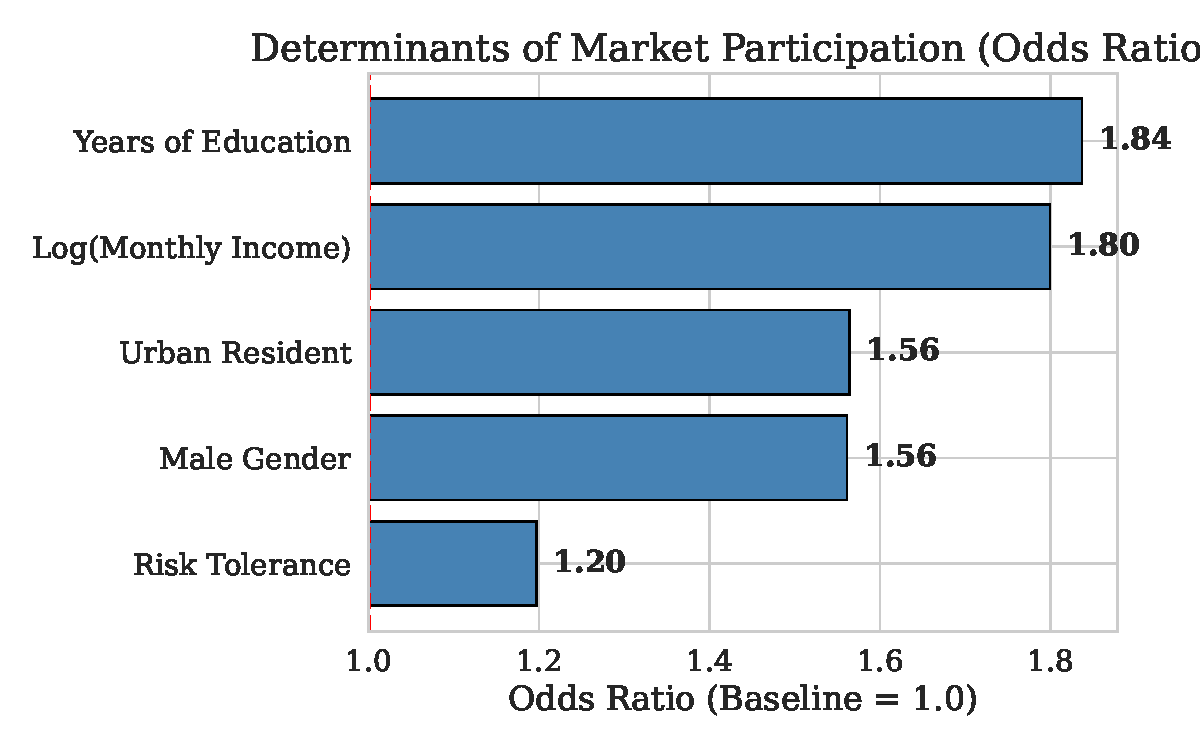
\includegraphics[height=0.8\textheight,keepaspectratio]{../figures/fig1_odds_ratios.pdf}
  \end{figure}
\end{frame}

% ── SLIDE 11: Finding 2 — Barrier archetypes ───────────────────────────────────
\begin{frame}{Finding 2: Three Archetypes of Non-Participation}
  K-means on 18 self-reported barriers identifies three profiles:
  \vspace{0.4em}
  \begin{block}{Trust-Deficient (46.3\%)}
    Persistent across income levels and urban cohorts.
    Requires institutional accountability: grievance redressal,
    IPF promotion, broker transparency.
  \end{block}
  \begin{block}{Knowledge-Gated (29.0\%)}
    Concentrated in rural areas and lowest income quartile.
    Needs geographically targeted vernacular literacy delivery.
  \end{block}
  \begin{block}{Fear-Driven (24.8\%)}
    Responds to loss-framing education and first-loss protection
    onramps (SGB, RBI Floating Rate Bonds).
  \end{block}
  \vspace{0.3em}
  A single awareness campaign cannot address all three.
\end{frame}

\begin{frame}{Finding 2: Archetype Demographics}
  \begin{figure}
    \centering
    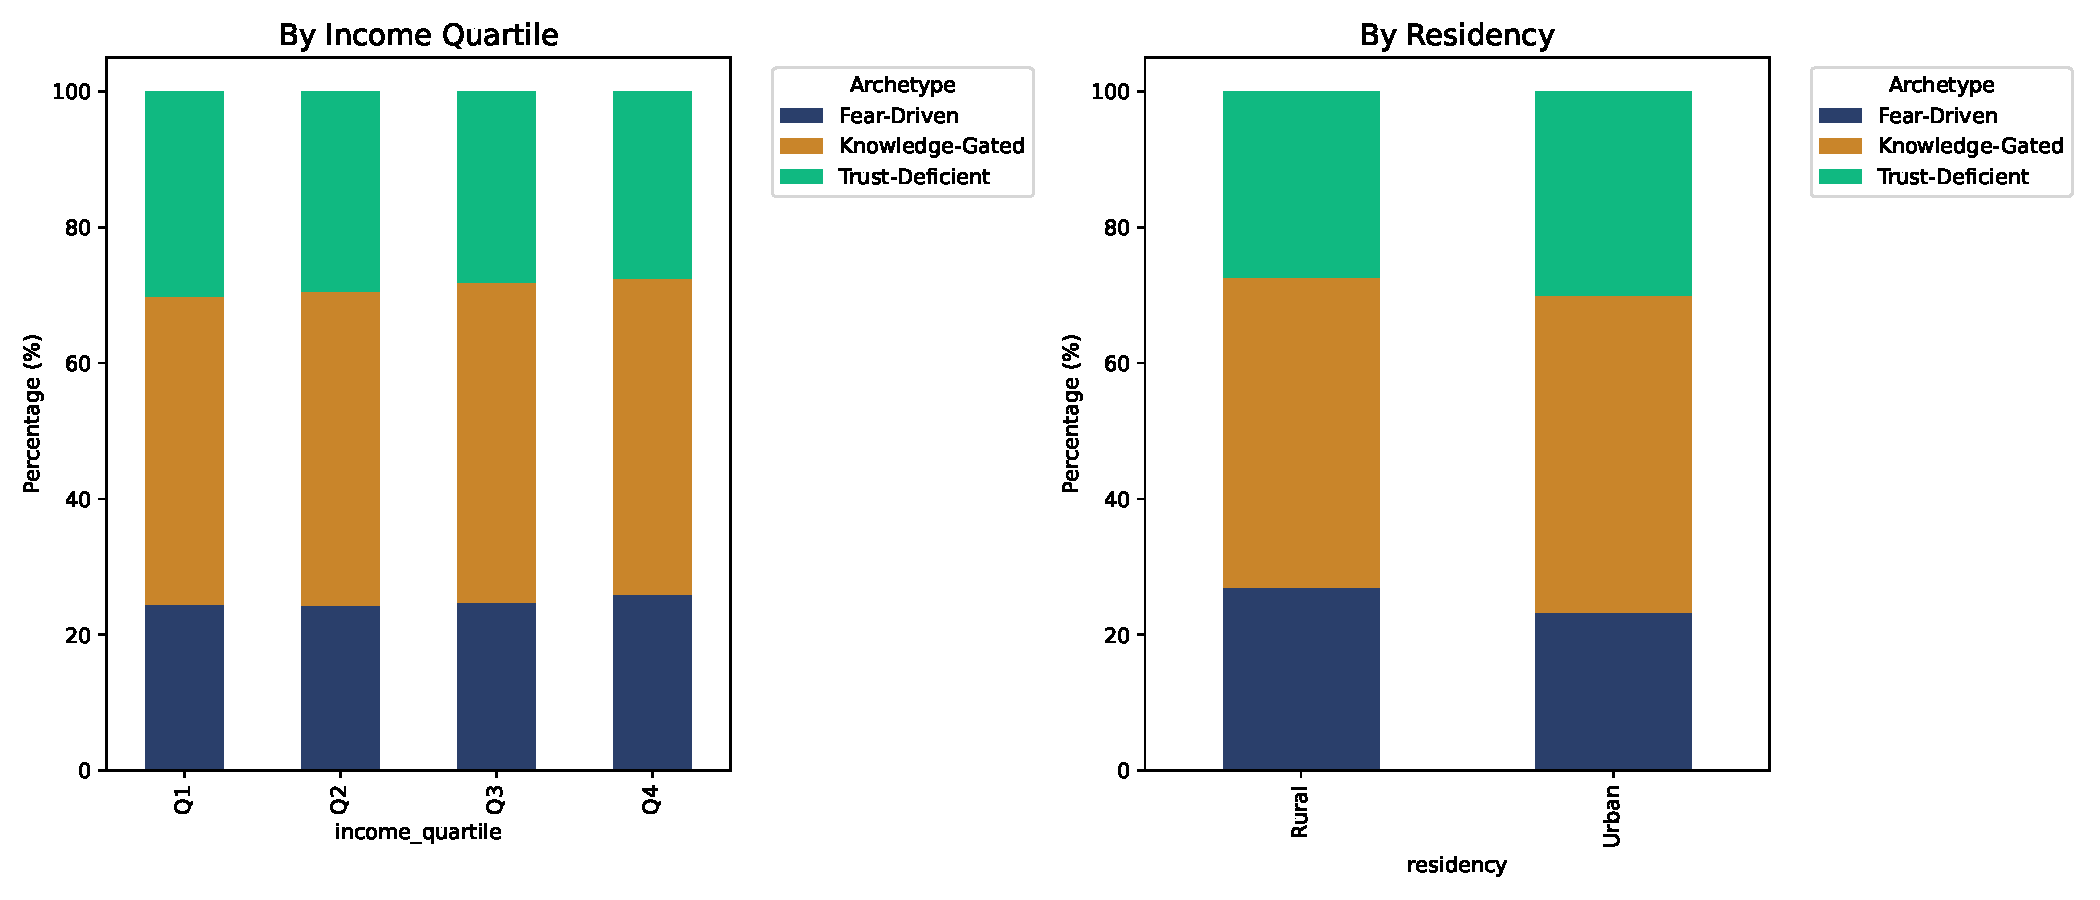
\includegraphics[height=0.8\textheight,keepaspectratio]{../figures/fig11_archetype_demographics.pdf}
  \end{figure}
\end{frame}

% ── SLIDE 14: Finding 3 — Behavioral traps ─────────────────────────────────────
\begin{frame}{Finding 3: Behavioral Traps Inside the Market}
  \textbf{Dunning-Kruger effect:}
  Investors with high perceived familiarity but low objective knowledge
  hold F\&O and crypto at significantly higher rates than calibrated peers.\\[0.8em]
  \textbf{Finfluencer pipeline:}
  5.0\% of investors cite social media as primary information source;
  this cohort is disproportionately quick-gains oriented relative to
  professionally-advised investors.\\[0.8em]
  \textbf{Goal-portfolio gap:}
  The ``Daily Trading'' cohort has a goal-portfolio consistency score
  of \alert{7.3\%}: they identify as speculators without holding the
  instruments that operationalize that strategy.\\[0.6em]
  These phenomena compound: aspirational investors, shaped by
  finfluencer content, are the segment most exposed to adverse outcomes.
\end{frame}

\begin{frame}{Finding 3: Dunning-Kruger and Holdings}
  \begin{figure}
    \centering
    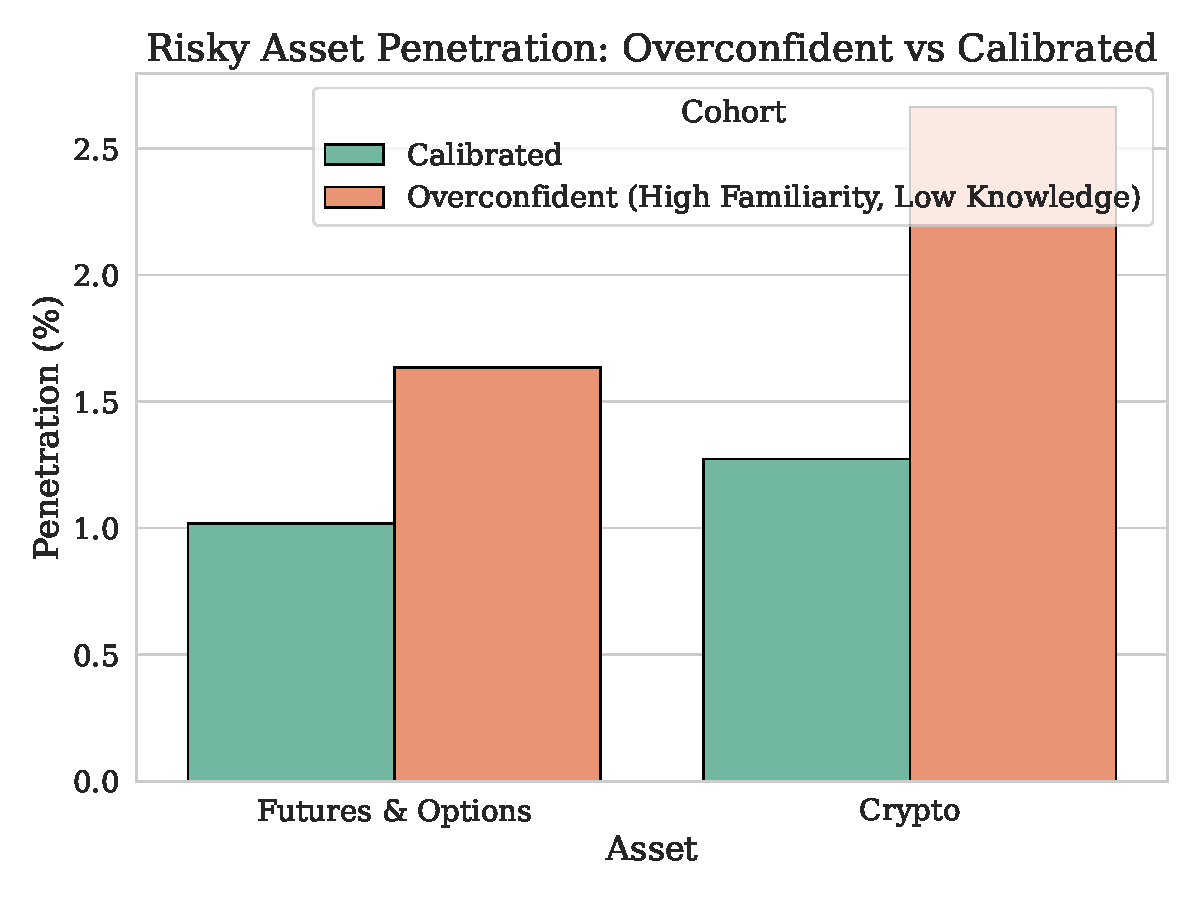
\includegraphics[height=0.8\textheight,keepaspectratio]{../figures/fig5_dunning_kruger.pdf}
  \end{figure}
\end{frame}

\begin{frame}{Finding 3: Goal-Portfolio Consistency}
  \begin{figure}
    \centering
    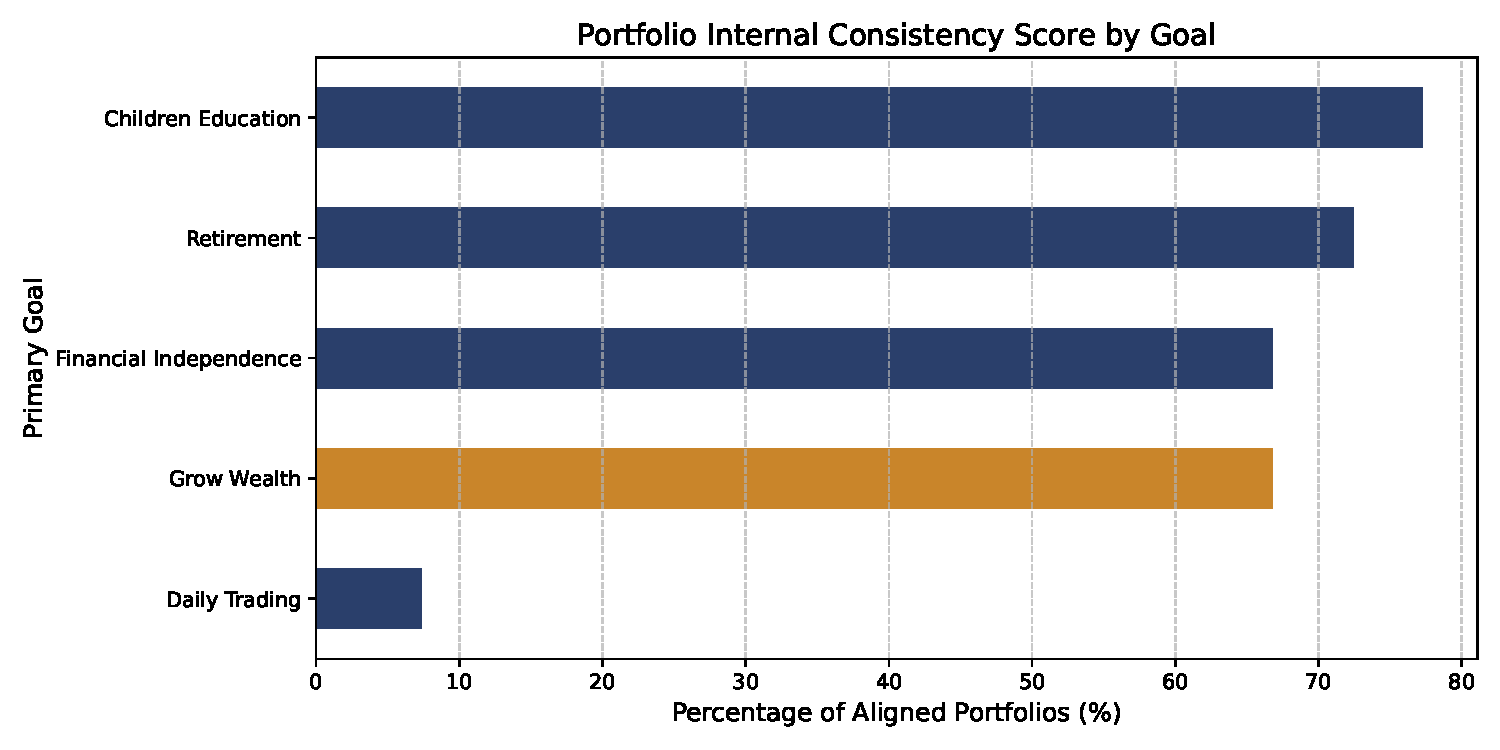
\includegraphics[height=0.8\textheight,keepaspectratio]{../figures/fig9_consistency_score.pdf}
  \end{figure}
\end{frame}

% ── SLIDE 17: Finding 4 — IEP ──────────────────────────────────────────────────
\begin{frame}{Finding 4: Investor Education Programme Impact}
  \textbf{2,768 investors (9.9\%)} cite SEBI or industry IEP as a
  top information source.\\[0.6em]
  \begin{center}
    \begin{tabular}{lcc}
      \toprule
      Metric & IEP & Non-IEP \\
      \midrule
      Knowledge score & \textbf{5.30} & 3.75 \\
      Products aware  & 10.23 & 10.23 \\
      Goal-based (\%) & \textbf{30.2} & 22.8 \\
      Quick gains (\%)& 21.7 & 23.3 \\
      Holds FDs (\%)  & 49.3 & \textbf{55.1} \\
      \bottomrule
    \end{tabular}
  \end{center}
  \vspace{0.6em}
  The 41\% knowledge advantage is specific to \emph{conceptual depth},
  not product breadth (awareness is near-identical).\\[0.4em]
  IEP functions as both a knowledge-deepening and a
  philosophical-reorientation intervention. Current reach: \alert{9.9\%}.
\end{frame}

\begin{frame}{Finding 4: IEP Analysis}
  \begin{figure}
    \centering
    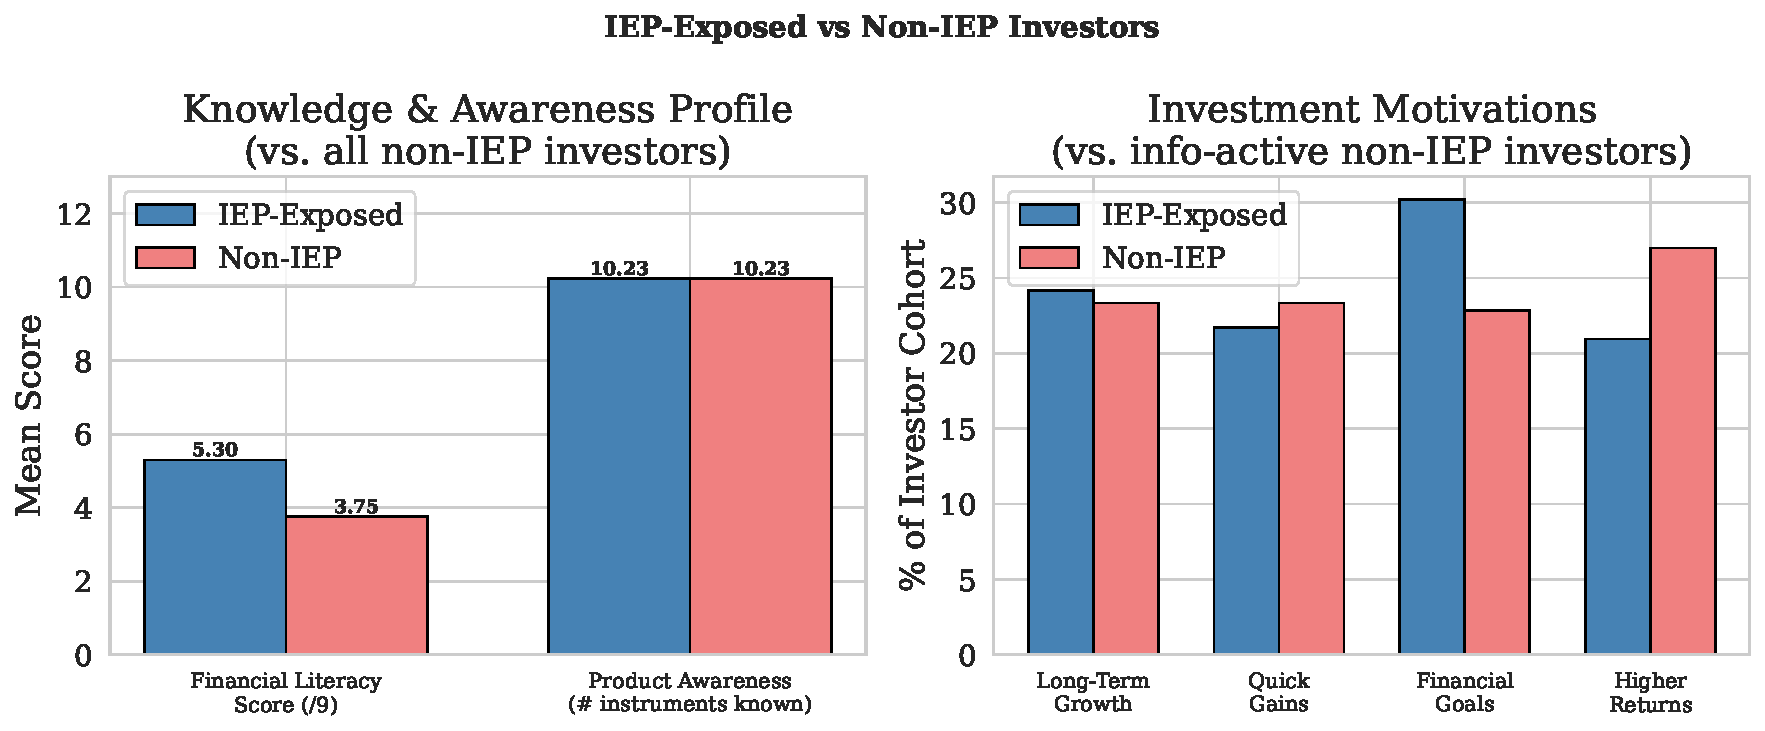
\includegraphics[height=0.7\textheight,keepaspectratio]{../figures/fig12_iep_analysis.pdf}
  \end{figure}
\end{frame}

% ── SLIDE 19: Predictive layer ────────────────────────────────────────────────
\begin{frame}{Predictive Layer: Machine Learning Results}
  \begin{center}
    \begin{tabular}{llc}
      \toprule
      Model & Task & AUC \\
      \midrule
      M1 & Participation & \textbf{0.814} \\
      M2 & Asset choice  & \textbf{0.820} \\
      M3 & Horizon       & 0.612 \\
      \bottomrule
    \end{tabular}
  \end{center}
  \vspace{0.8em}
  \textbf{Feature importance shift:}\\
  At the entry layer, \emph{product awareness} dominates.
  Inside the market, \emph{perceived familiarity} and
  \emph{objective knowledge} take over.\\[0.6em]
  Investment horizon (M3) is the hardest prediction,
  consistent with it being driven by situational factors
  outside a cross-sectional feature space.\\[0.6em]
  All three models include \texttt{n\_products\_aware}
  alongside demographic and behavioral features.
\end{frame}

\begin{frame}{Predictive Layer: Feature Importance}
  \begin{figure}
    \centering
    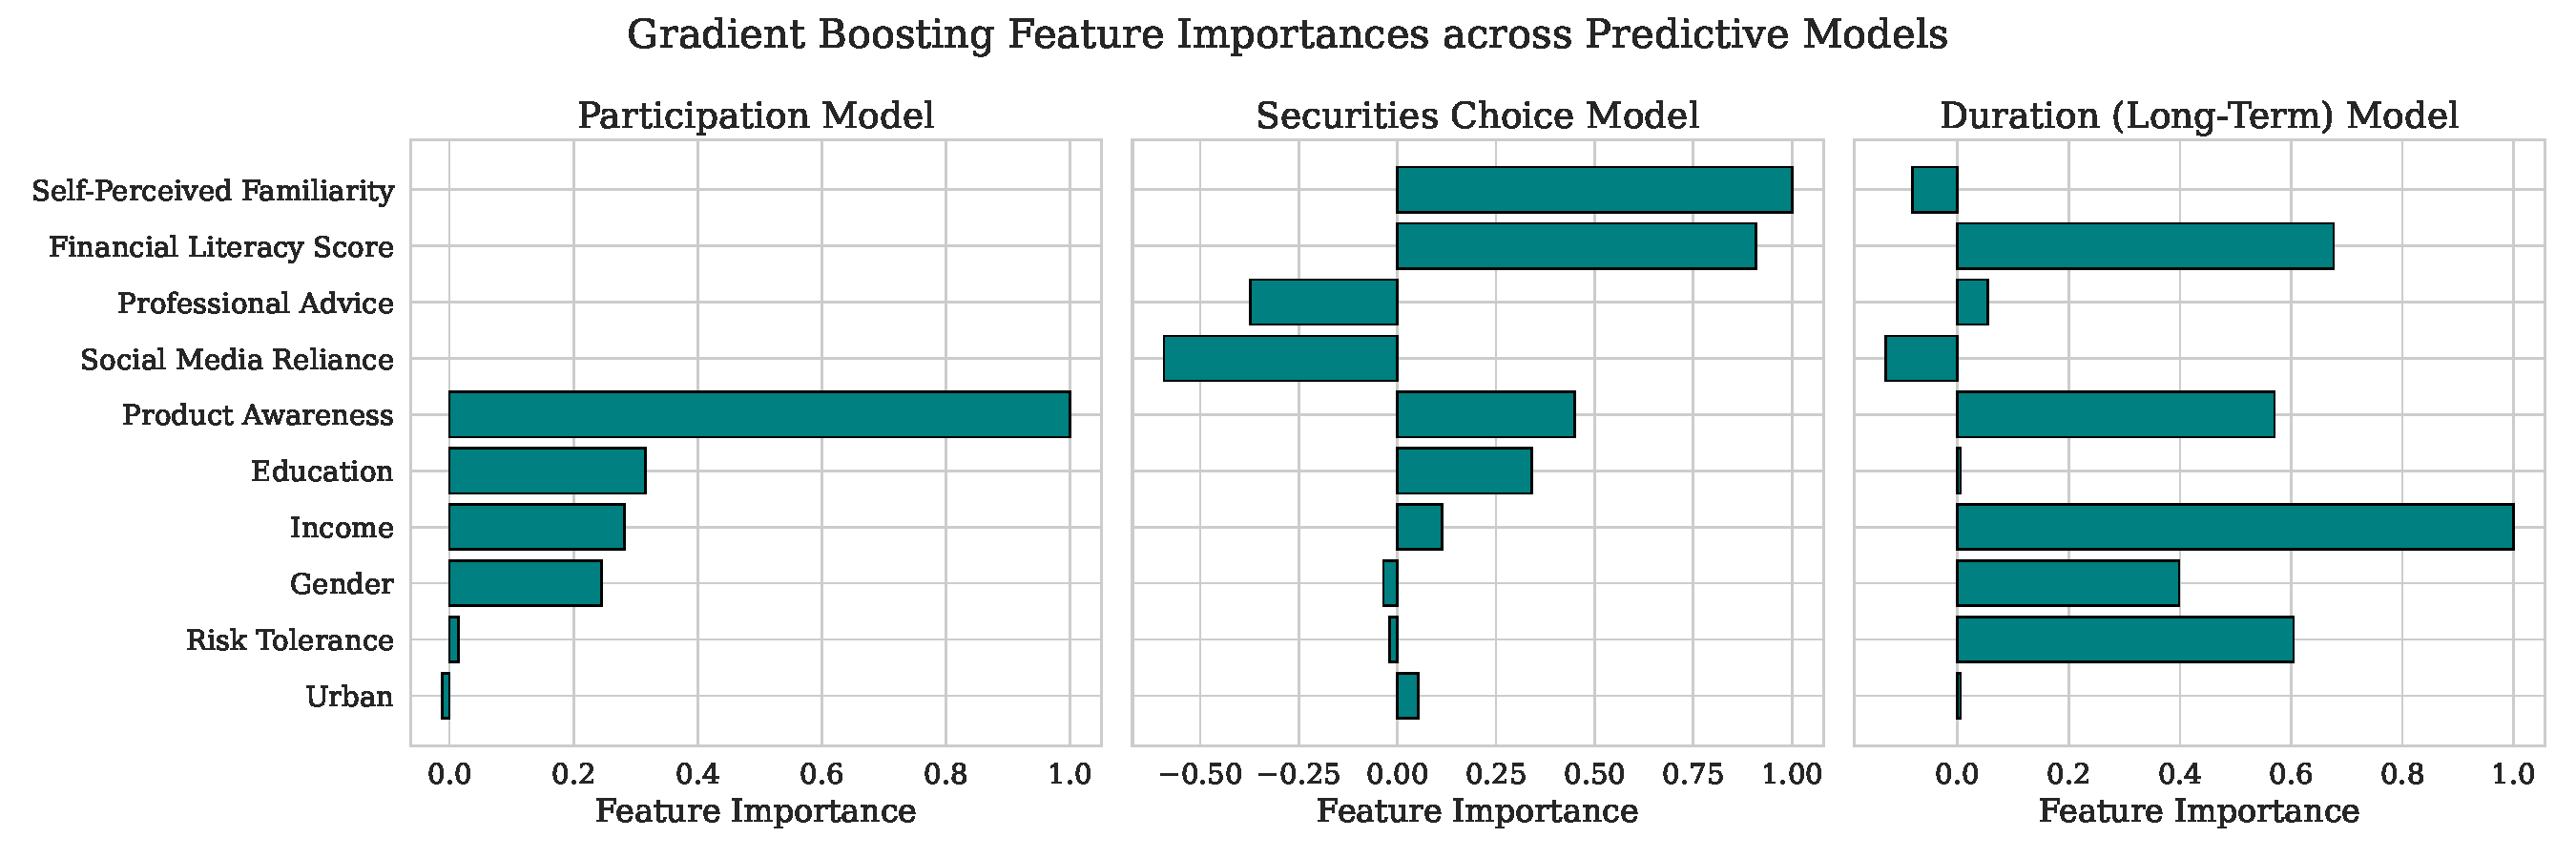
\includegraphics[height=0.6\textheight,keepaspectratio]{../figures/fig7_predictive_importance.pdf}
  \end{figure}
  \vfill
  \centering
  \scriptsize
  \textit{*Note: Negative permutation importance indicates high-variance predictors (e.g., social media usage) 
  that may appear noisy when shuffled individually. However, HistGradientBoosting utilizes these 
  features for critical conditional interactions; their removal breaks high-precision decision branches, 
  leading to lower aggregate AUC.}
\end{frame}


% ── SLIDE 21: Policy ──────────────────────────────────────────────────────────
\begin{frame}{Policy Recommendations}
  \begin{columns}[T]
    \begin{column}{0.48\textwidth}
      \textbf{A. Prioritize product awareness}\\
      OR = 2.22; campaigns should name specific instruments
      (MF, ETF, SIP) for North and South zones.\\[0.4em]

      \textbf{B. Segment non-investor interventions}\\
      Trust-Deficient: regulatory transparency.
      Knowledge-Gated: vernacular rural delivery.
      Fear-Driven: first-loss protection onramps.\\[0.4em]

      \textbf{C. Scale IEP reach}\\
      From 9.9\% to employer mandates and Jan Dhan partnerships.
      Content should emphasize conceptual depth, not procedural literacy
      (KYC awareness is already high). Goal-aligned investors show
      72--77\% portfolio consistency, confirming goal-based framing works.
    \end{column}
    \begin{column}{0.48\textwidth}
      \textbf{D. Close the gender gap}\\
      OR = 1.53 for male gender after full controls. SHG-linked
      investment collectives, women-targeted IEP content,
      lower minimum investment thresholds.\\[0.4em]

      \textbf{E. Regulate finfluencers}\\
      5\% usage associated with quick-gains orientation.
      Mandatory qualification disclosure, prohibited performance claims,
      platform liability for unregistered advice.\\[0.4em]

      \textbf{F. Gate derivatives on objective literacy}\\
      Overconfident investors and aspirational daily traders (7.3\%
      consistency) reach leveraged instruments without adequate knowledge.
      Replace self-certification with a brief objective literacy assessment.
    \end{column}
  \end{columns}
\end{frame}

\begin{frame}{Implementation: Stockbroker Sales AI}
  \begin{figure}
    \centering
    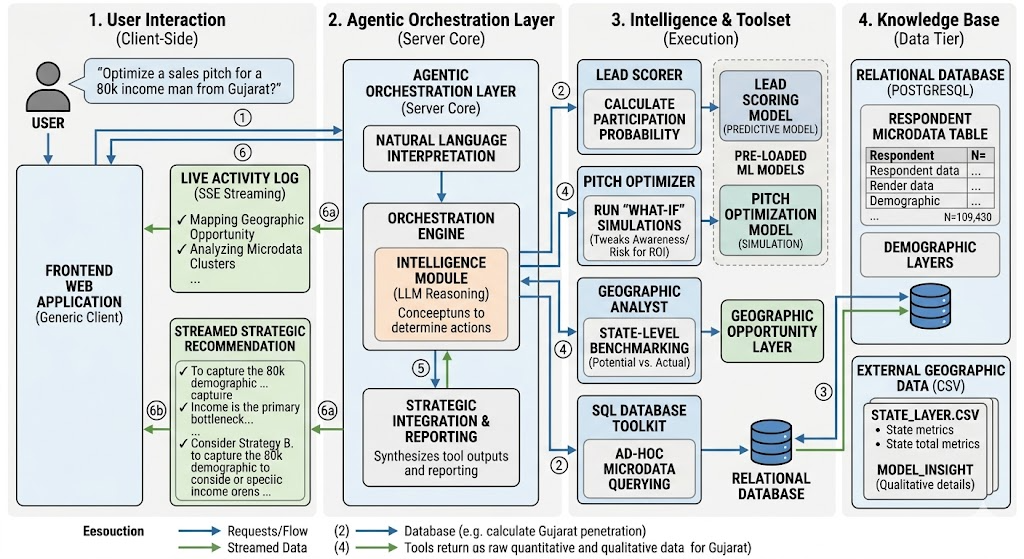
\includegraphics[width=1.035\linewidth]{../figures/ai_layer.png}
  \end{figure}
\end{frame}

% ── Appendix ──────────────────────────────────────────────────────────────────
\appendix

\begin{frame}{Appendix: Holdings by Income Quartile}
  \begin{figure}
    \centering
    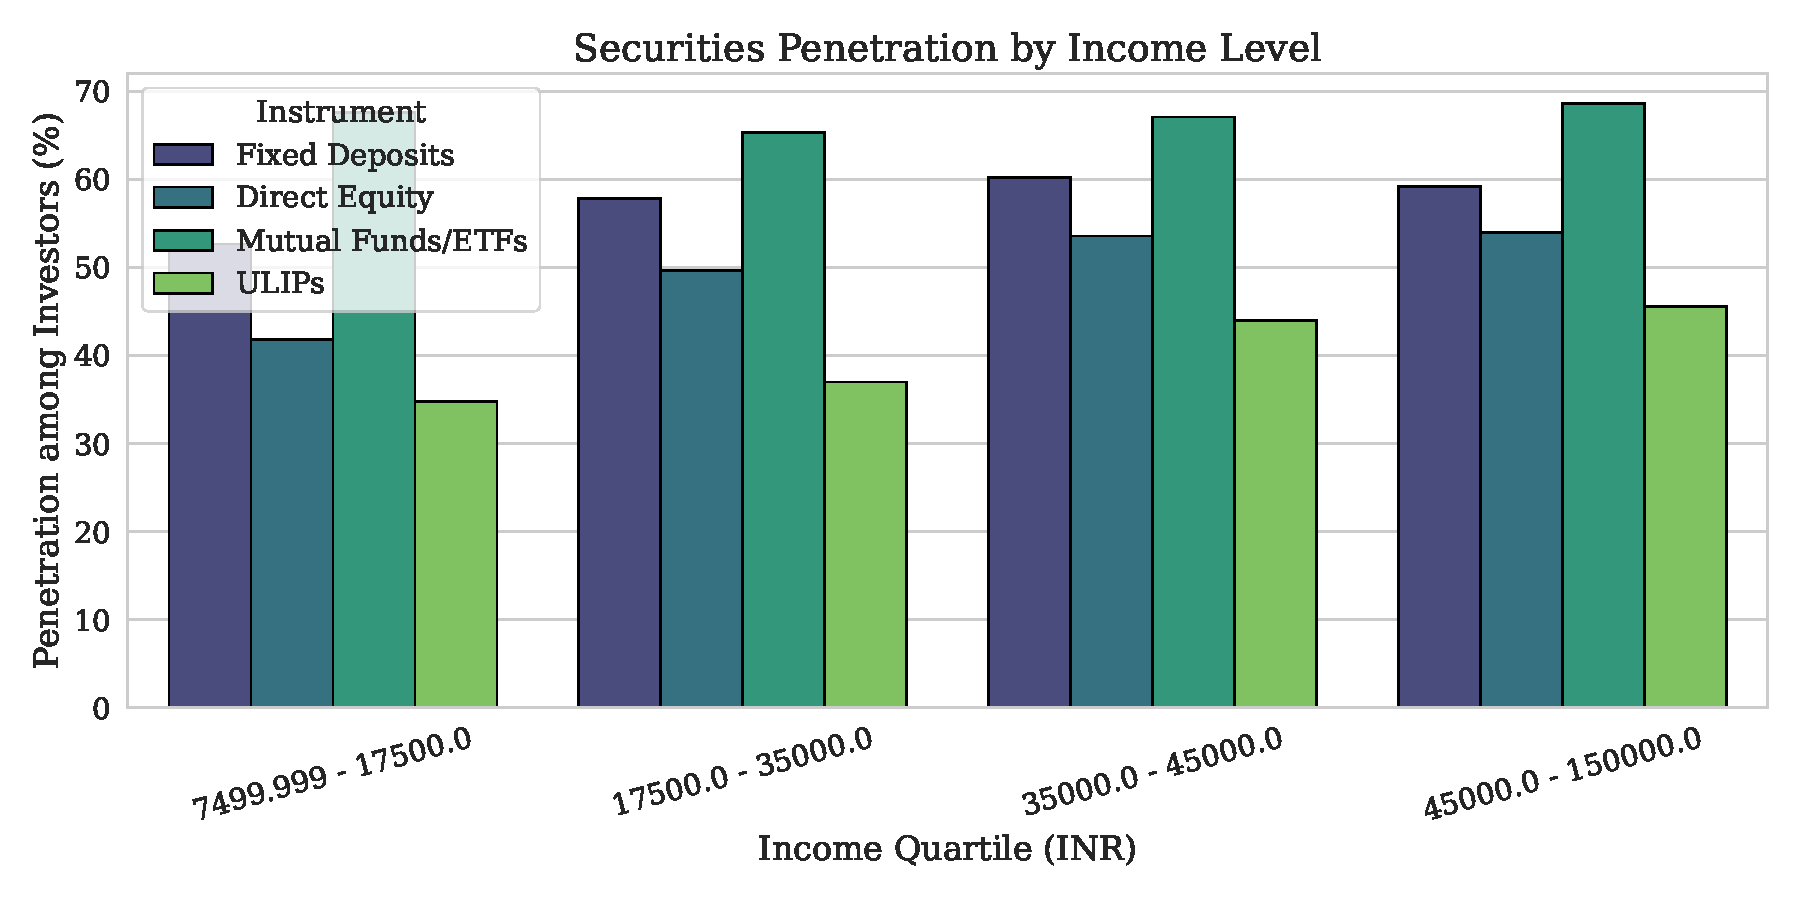
\includegraphics[width=0.75\linewidth]{../figures/fig3_securities_income.pdf}
    \caption*{Market-linked instruments scale sharply with wealth.}
  \end{figure}
\end{frame}

\begin{frame}{Appendix: Investment Horizons by Asset Class}
  \begin{figure}
    \centering
    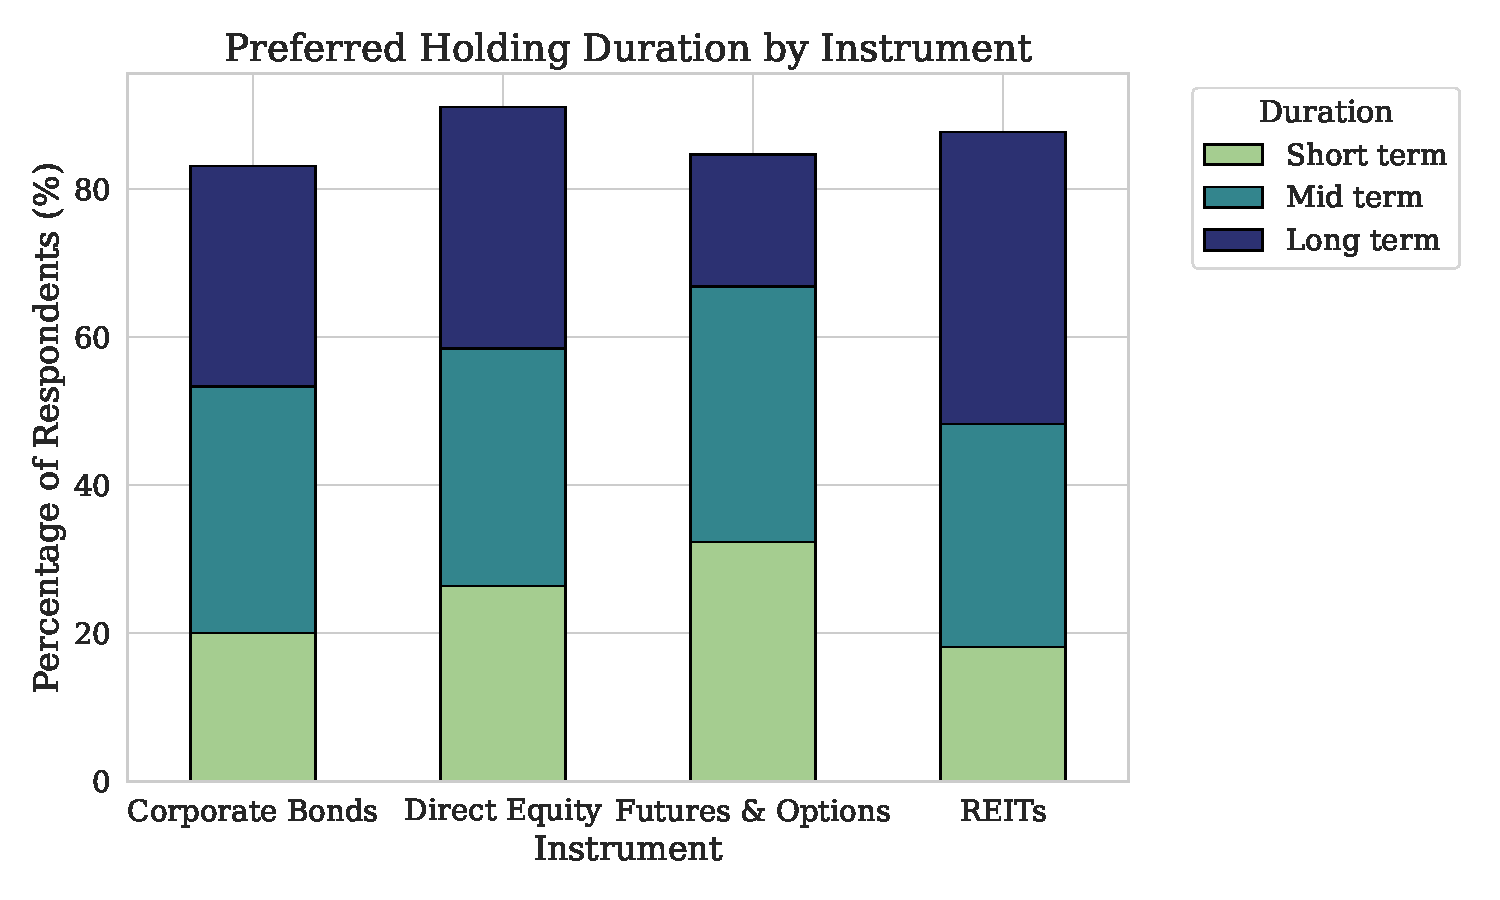
\includegraphics[width=0.75\linewidth]{../figures/fig4_duration.pdf}
    \caption*{Equities and MFs held long-term; derivatives skew short-term.}
  \end{figure}
\end{frame}

\begin{frame}{Appendix: Barrier Archetype Profiles (Centroids)}
  \begin{figure}
    \centering
    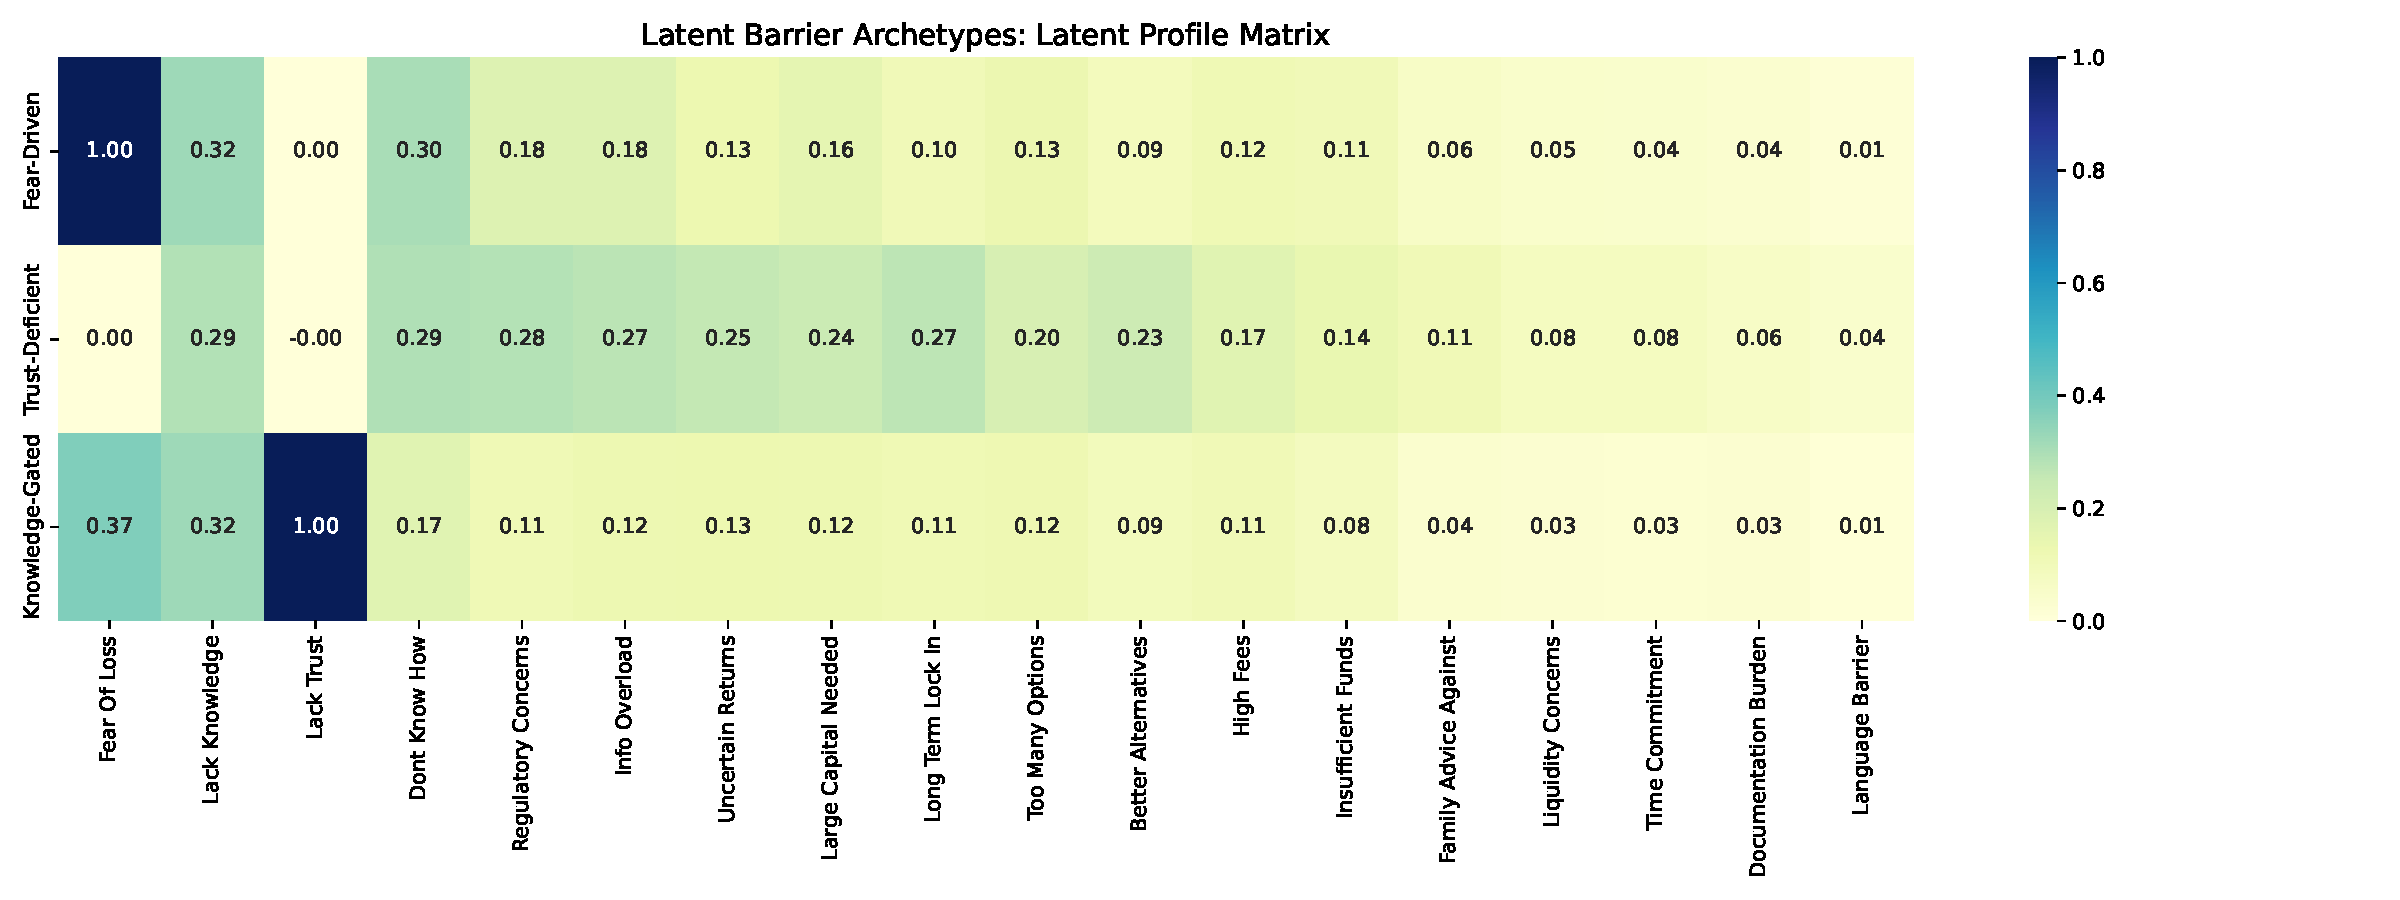
\includegraphics[width=0.9\linewidth]{../figures/fig10_barrier_archetypes_heatmap.pdf}
    \caption*{Centroid matrix of the 18-dimensional barrier space. Values represent the probability of each barrier being present in the archetype profile.}
  \end{figure}
\end{frame}

\begin{frame}{Appendix: Archetype Defining Peaks}
  \begin{figure}
    \centering
    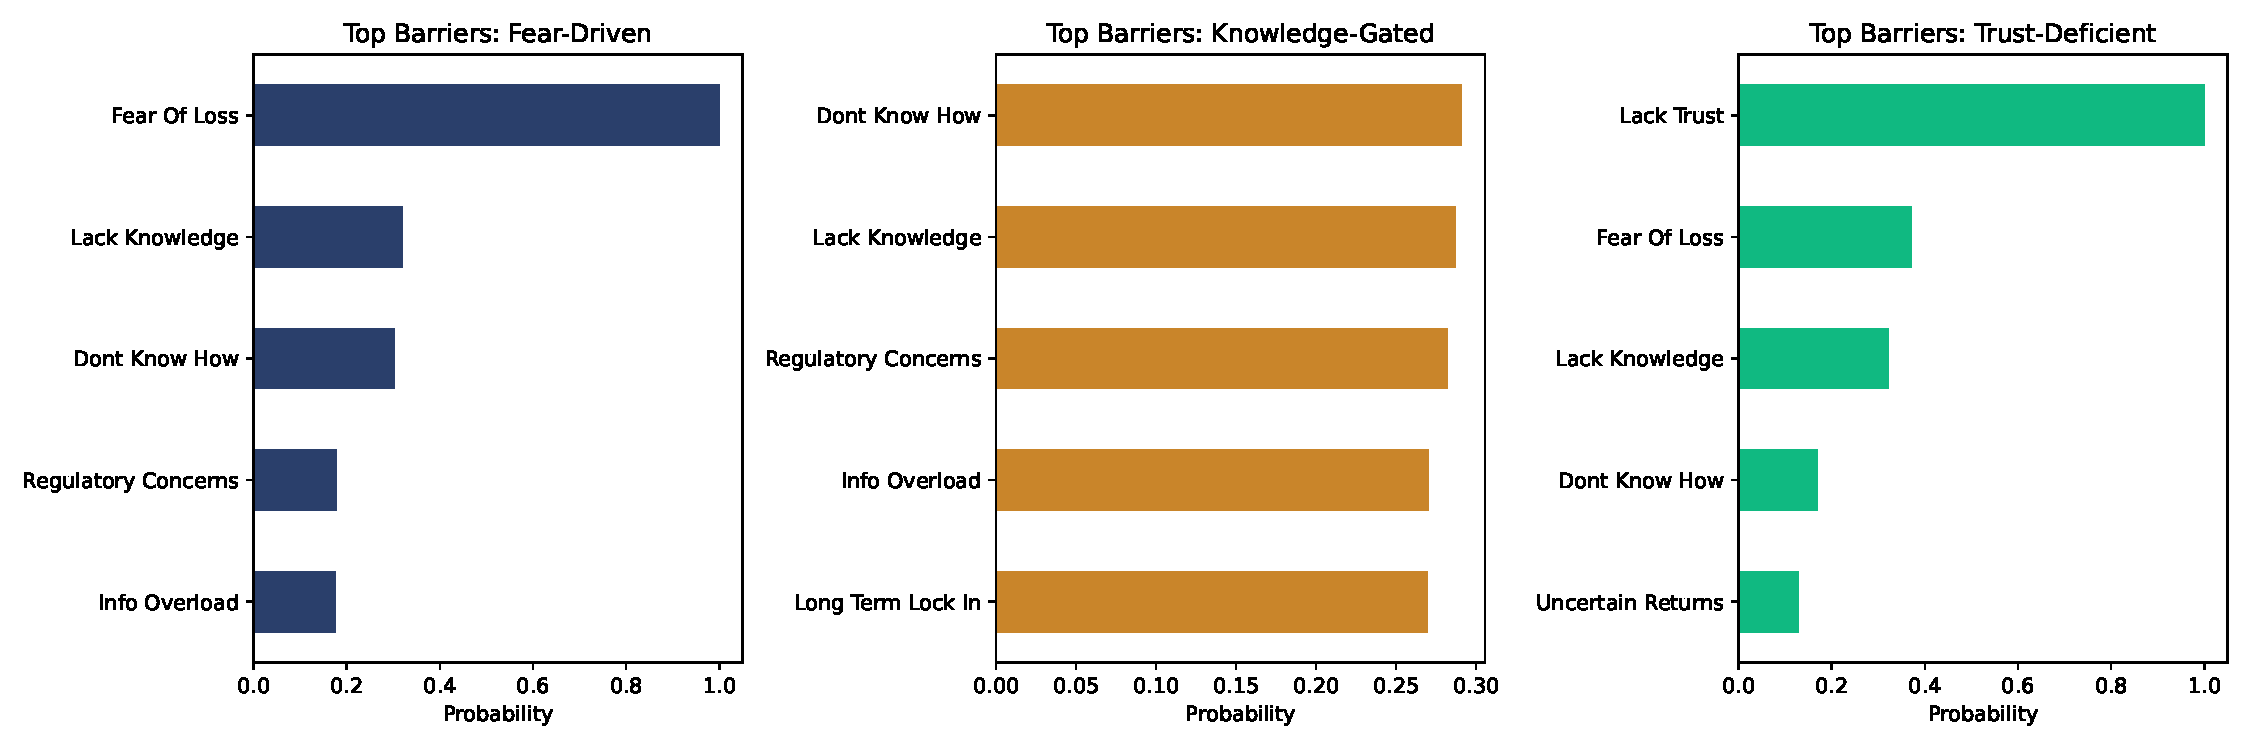
\includegraphics[width=\linewidth]{../figures/fig15_archetype_peaks.pdf}
    \caption*{Top 5 barriers for each archetype. These peaks define the strategic naming: Fear-Driven (Fear of Loss), Knowledge-Gated (Lack Knowledge), and Trust-Deficient (Lack Trust).}
  \end{figure}
\end{frame}


\begin{frame}{Appendix: Full Logistic Regression Table}
  \centering
  \small
  \begin{tabular}{lcccc}
    \toprule
    \textbf{Predictor} & \textbf{OR} & \textbf{95\% CI} & $z$ & Sig. \\
    \midrule
    Product Awareness & 2.218 & [2.166, 2.272] & 65.2 & *** \\
    Log(Income)       & 1.603 & [1.564, 1.643] & 37.4 & *** \\
    Education (yrs)   & 1.556 & [1.518, 1.594] & 35.6 & *** \\
    Male              & 1.526 & [1.490, 1.564] & 33.9 & *** \\
    Urban             & 1.455 & [1.422, 1.489] & 32.0 & *** \\
    Risk Tolerance    & 1.170 & [1.145, 1.196] & 14.0 & *** \\
    Millennial        & 1.124 & [1.098, 1.151] &  9.8 & *** \\
    Gen X             & 0.993 & [0.969, 1.017] & $-$0.6 & \\
    Baby Boomer       & 0.907 & [0.881, 0.934] & $-$6.6 & *** \\
    North             & 0.850 & [0.825, 0.876] & $-$10.7 & *** \\
    South             & 0.842 & [0.816, 0.869] & $-$10.7 & *** \\
    West              & 1.021 & [0.989, 1.054] &  1.3 & \\
    \midrule
    \multicolumn{5}{l}{$N = 97{,}626$ \quad McFadden $R^2 = 0.290$ \quad *** $p < 0.001$, HC3 robust SE} \\
    \bottomrule
  \end{tabular}
\end{frame}

\end{document}
